\documentclass[compose]{exam-n}

\usepackage{graphics}
\graphicspath{{fig/}}

\begin{document}

\begin{question}{20}  \author{Reginald Q Whimsy}
% Have a blank line here, to check that the question number remains
% nicely lined up, even if there are lines between the environment
% opening and the text.

First, \emph{admire} the restful picture of a spiral in Fig.\ \ref{f:spiral},
included as a graphic.  Fully zenned up?  Then let us begin\dots.
\begin{figure}
\ifbigfont
  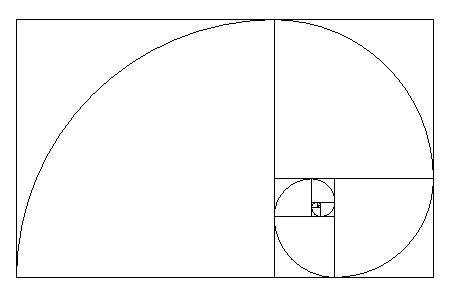
\includegraphics[width=\textwidth]{spiral}
\else
  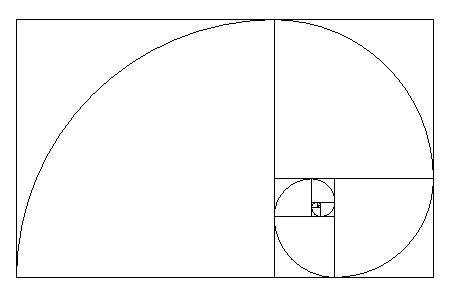
\includegraphics{spiral}
\fi
\caption{\label{f:spiral}A spiral}
\end{figure}

\part Show that, under the action of gravity alone, the scale size
of the Universe varies according to
\begin{equation}
\ddot{R}=-\frac{4\pi G \rho_0}{3R^2}
\end{equation}
\partmarks*{4}
and that, consequently,
\begin{equation*}
\dot{R}^2=-\frac{8\pi G \rho_0}{3R}=-K.
\partmarks*{3}
\end{equation*}

Express $K$ in terms of the present values of the Hubble constant
$H_0$ and of the density parameter $\Omega_0$.
\partmarks{3}
\begin{solution}
This can be solved by \emph{remembering} the solution
\partmarks{3}
\end{solution}

\part In the early Universe, the relation between time and
temperature has the form
\begin{equation*}
t=\sqrt{\frac{3c^2}{16\pi G g_{\rm eff}a}}\frac{1}{T^2},
\end{equation*}
where $a$  is the radiation constant. Discuss the assumptions
leading to this equation, but do not carry out the mathematical
derivation.  Discuss the meaning of the factor $g_{\rm eff}$ , and
find its value just before and after annihilation of electrons and
positrons.
\partmarks{6}
\begin{solution}
Before, well, geee; after\dots kazamm!
\end{solution}

\part
Explain how the present-day neutron/proton ratio was established
by particle interactions in the Early Universe. How is the ratio
of deuterium to helium relevant to the nature of dark matter?  It is
\emph{crucially vital} to note
that Table~\ref{t:dullness} is of absolutely no relevance to this question.
\begin{table}
\begin{tabular}{r|l}
Column 1&and row 1\\
More content&in row 2
\end{tabular}
\caption{\label{t:dullness}A remarkably dull table}
\end{table}
Finis.
\begin{questiondata}
Hubble's law: $v=H_0 D$
\end{questiondata}
\partmarks{4}
\begin{solution}
Explanations are superfluous; all that is, is.
\begin{table}
\begin{tabular}{r|l}
First rows&are premier\\
subsequent rows&are of secondary interest
\end{tabular}
\caption{\label{t:dullnessII}A table o'erbrimming with otioseness}
\end{table}
In addition, Table~\ref{t:dullnessII} adds nothing to the discussion,
adds nothing to our understanding of our place in the cosmos, but it
\emph{does} contribute slightly to the heat-death of the universe (can
you work out how many deuterium nuclei decayed during the typing of
this table?).
\end{solution}
\end{question}
\end{document}
